% vim: ts=4 sts=4 sw=4 et tw=75
\chapter{Notation}
\label{chap:notation}
\begin{quote}
    Perhaps of all the creations of man language is the most astonishing
    (惊讶的).
\end{quote}
\begin{quotesrc}
    Giles Lytton Strachey, \bookname{Words and Poetry}
\end{quotesrc}

The right language can make all the difference in how easy it is to write a
program. This is why a practicing programmer's arsenal holds not only
general-purpose languages like C and its relatives, but also programmable
shells, scripting languages, and lots of application-specific languages

The power of good notation reaches beyond traditional programming into
specialized problem domains. Regular expressions let us write compact (if
occasionally cryptic (神秘的)) definitions of classes of strings; HTML lets
us define the layout of interactive documents, often using embedded
programs in other languages such as JavaScript; Postscript expresses an
entire document -- this book, for example -- as a stylized program.
Spreadsheets and word processors often include programming languages like
Visual Basic to evaluate expressions, access information, or control
layout.

If you find yourself writing too much code to do a mundane (平凡的) job, or
if you have trouble expressing the process comfortably, maybe you're using
the wrong language. If the right language doesn't yet exist, that might be
an opportunity to create it yourself. Inventing a language doesn't
necessarily mean building the successor to Java; often a thorny (多刺的)
problem can be cleared up by a change of notation. Consider the format
strings in the \verb'printf' family, which are a compact and expressive way
to control the display of printed values.

In this chapter, we'll talk about how notation can solve problems, and
demonstrate some of the techniques you can use to implement your own
special-purpose languages. We'll even explore the possibilities of having
one program write another program, an apparently extreme use of notation
that happens more often, and is far easier to do, than many programmers
realize.

\section{Formatting Data}
\label{sec:formatting_data}

There is always a gap between what we want to say to the computer ("solve
my problem") and what we are required to say to get a job done. The
narrower this gap, the better. Good notation makes it easier to say what we
want and harder to say the wrong thing by mistake. Sometimes, good notation
can provide new insight (见识, 洞察), allowing us to solve problems that
seemed too difficult, or even lead us to new discoveries.

\textbf{\texttt{Little languages}} are specialized notations for narrow
domains. They not only provide a good interface but also help organize the
program that implements them. The \verb'printf' control sequences are a
good example:
\begin{wellcode}
    printf("%d %6.2f %-10.10s\n", i, f, s);
\end{wellcode}

Each \verb'%' in the format string signals a place to interpolate (插入)
the value of the next \verb'printf' argument; after some optional flags and
field widths, the terminating letter says what kind of parameter to expect.
This notation is compact, intuitive, and easy to write, and the
implementation is straightforward. The alternatives in C++
(\verb'iostream') and Java (\verb'java.io') seem more awkward (笨拙) since
they don't provide special notation, although they extend to user-defined
types and offer type-checking.

Some non-standard implementations of \verb'printf' let you add your own
conversions to the built-in set. This is convenient if you have other data
types that need output conversion. For example, a compiler might use
\verb'%L' for line number and file name; a graphics system might use
\verb'%P' for a point and \verb'%R' for a rectangle. The cryptic string of
letters and numbers for retrieving stock quotes (股价报价) that we saw in
Chapter \ref{chap:interface} was in the same spirit, a compact notation for
arranging (编排) combinations of stock data.

We can synthesize similar examples in C and C++. Suppose we want to send
packets containing various combinations of data types from one system to
another.  As we saw in Chapter \ref{chap:portability}, the cleanest
solution may be to convert to a textual representation. For a standard
network protocol, though, the format is likely to be binary for reasons of
efficiency or size. How can we write the packet-handling code to be
portable, efficient, and easy to use?

To make this discussion concrete, imagine that we plan to send packets of
8-bit, 16-bit, and 32-bit data items from system to system. ANSI C says
that we can always store at least 8 bits in a \verb'char', 16 bits in a
\verb'short', and 32 bits in a \verb'long', so we will use these data types
to represent our values. There will be many types of packets; packet type 1
might have a 1-byte type specifier, a 2-byte count, a 1-byte value and a
4-byte data item:
\begin{center}
    \begin{tikzpicture}
        \pgfmathsetmacro\width{1.5};

        \draw (0, 0) -- (\width * 8, 0);
        \draw (0, 1) -- (\width * 8, 1);
        \foreach \i in {0, ..., 8}
        \draw (\i * \width, 0) -- (\i * \width, 1);

        \newcounter{j};
        \setcounter{j}{0};
        \foreach \ind/\data in { 0/\texttt{0x01}, 1/\texttt{cnt$_1$},
            2/\texttt{cnt$_0$}, 3/\texttt{val}, 4/\texttt{data$_3$},
            5/\texttt{data$_2$}, 6/\texttt{data$_1$},
            7/\texttt{data$_0$}} {

            \node at (\arabic{j} * \width + \width / 2, 0.5)
                {\data};
            \addtocounter{j}{1};
        }
    \end{tikzpicture}
\end{center}
Packet type 2 might contain a short and two long data words:
\begin{center}
    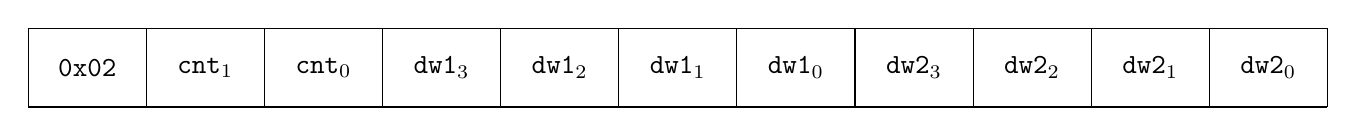
\begin{tikzpicture}
        \pgfmathsetmacro\width{1.5};

        \draw (0, 0) -- (\width * 11, 0);
        \draw (0, 1) -- (\width * 11, 1);
        \foreach \i in {0, ..., 11}
        \draw (\i * \width, 0) -- (\i * \width, 1);

        \setcounter{j}{0};
        \foreach \ind/\data in { 0/\texttt{0x02}, 1/\texttt{cnt$_1$},
            2/\texttt{cnt$_0$}, 3/\texttt{dw1$_3$},
            4/\texttt{dw1$_2$}, 5/\texttt{dw1$_1$},
            6/\texttt{dw1$_0$}, 7/\texttt{dw2$_3$}, 8/\texttt{dw2$_2$},
            9/\texttt{dw2$_1$}, 10/\texttt{dw2$_0$}} {

            \node at (\arabic{j} * \width + \width / 2, 0.5)
                {\data};
            \addtocounter{j}{1};
        }
    \end{tikzpicture}
\end{center}

One approach is to write pack and unpack functions for each possible packet
type:
\begin{wellcode}
    int pack_type1(unsigned char *buf, unsigned short count,
            unsigned char val, unsigned long data)
    {
        unsigned char *bp;

        bp = buf;
        *bp++ = 0x01;
        *bp++ = count >> 8;
        *bp++ = count;
        *bp++ = val;
        *bp++ = data >> 24;
        *bp++ = data >> 16;
        *bp++ = data >> 8;
        *bp++ = data;
        return bp - buf;
    }
\end{wellcode}
For a realistic protocol, there will be dozens of such routines, all
variations on a theme. The routines could be simplified by using macros or
functions to handle the basic data types (\verb'short', \verb'long', and so
on), but even so, such repetitive code is easy to get wrong, hard to read,
and hard to maintain.

The inherent (固有的) repetitiveness (重复性) of the code is a clue that
notation can help.  Borrowing the idea from \verb'printf', we can define a
tiny specification language in which each packet is described by a brief
string that captures the packet layout.  Successive elements of the packet
are encoded with \verb'c' for an 8-bit character, \verb's' for a 16-bit
short integer, and \verb'l' for a 32-bit long integer. Thus, for example,
the packet type 1 built by our example above, including the initial type
byte, might be described by the format string \verb'cscl'. Then we can use
a single pack function to create packets of any type; this packet would be
created with
\begin{wellcode}
    pack(buf, "cscl", 0x01, count, val, data);
\end{wellcode}
Because our format string contains only data definitions, there's no need
for the \verb'%' character used by \verb'printf'.

In practice, information at the beginning of the packet might tell the
recipient (接受者) how to decode the rest, but we'll assume the first byte
of the packet can be used to determine the layout. The sender encodes the
data in this format and ships it; the receiver reads the packet, picks off
the first byte, and uses that to decode what follows.

Here is an implementation of \verb'pack', which fills \verb'buf' with the
encoded representation of its arguments as determined by the format. We
make all values unsigned, including the bytes in the packet buffer, to
avoid sign-extension problems.  We also use some conventional
\verb'typedef's to keep the declarations short:
\begin{wellcode}
    typedef unsigned char   uchar;
    typedef unsigned short  ushort;
    typedef unsigned long   ulong;
\end{wellcode}
Like \verb'sprintf', \verb'strcpy', and similar functions, \verb'pack'
assumes that the buffer is big enough to hold the result; it is the
caller's responsibility to ensure this. There is also no attempt to detect
mismatches between the format and the argument list.
\begin{wellcode}
    #include <stdarg.h>

    /* pack: pack binary items into buf, return length */
    int pack(uchar *buf, char *fmt, ...)
    {
        va_list args;
        char    *p;
        uchar   *bp;
        ushort  s;
        ulong   l;
        bp = buf;
        va_start(args, fmt);
        for (p = fmt; *p != '\0'; p++) {
            switch (*p) {
            case 'c':   /* char */
                *bp++ = va_arg(args, int);
                break;
            case 's':   /* short */
                s = va_arg(args, int);
                *bp++ = s >> 8;
                *bp++ = s;
                break;
            case 'l':   /* long */
                l = va_arg(args, ulong);
                *bp++ = l >> 24;
                *bp++ = l >> 16;
                *bp++ = l >> 8;
                *bp++ = l;
                break;
            default:    /* illegal type character */
                va_end(args);
                return -1;
            }
        }
        va_end(args);
        return bp - buf;
    }
\end{wellcode}

The \verb'pack' routine uses the \verb'stdarg.h' header more extensively
than \verb'eprintf' did in Chapter \ref{chap:interface}. The successive
arguments are extracted using the macro \verb'va_arg', with first operand
the variable of type \verb'va_list' set up by calling \verb'va_start' and
second operand the type of the argument (this is why \verb'va_arg' is a
macro, not a function).  When processing is done, \verb'va_end' must be
called. Although the arguments for \verb"'c'" and \verb"'s'" represent
\verb'char' and \verb'short' values, they must be extracted as \verb'int's
because C promotes (提升) \verb'char' and \verb'short' arguments to
\verb'int' when they are represented by an ellipsis \verb'...'  parameter.

Each \verb'pack_type' routine will now be one line long, marshaling
(封装处理) its arguments into a call of \verb'pack':
\begin{wellcode}
    /* pack_type1: pack format 1 packet */
    int pack_type1(uchar *buf, ushort count, uchar val, ulong data)
    {
        return pack(buf, "cscl", 0x01, count, val, data);
    }
\end{wellcode}

To unpack, we can do the same thing: rather than write separate code to
crack each packet format, we call a single \verb'unpack' with a format
string. This centralizes the conversion in one place:
\begin{wellcode}
    /* unpack: unpack packed items from buf, return length */
    int unpack(uchar *buf, char *fmt, ...)
    {
        va_list args;
        char    *p;
        uchar   *bp, *pc;
        ushort  *ps;
        ulong   *pl;

        bp = buf;
        va_start(args, fmt);
        for (p = fmt; *p != '\0'; p++) {
            switch (*p) {
            case 'c':   /* char */
                pc = va_arg(args, uchar *);
                *pc = *bp++;
                break;
            case 's':   /* short */
                ps = va_arg(args, ushort *);
                *ps = *bp++ << 8;
                *ps |= *bp++;
                break;
            case 'l':   /* long */
                pl = va_arg(args, ulong *);
                *pl = *bp++ << 24;
                *pl |= *bp++ << 16;
                *pl |= *bp++ << 8;
                *pl |= *bp++;
                break;
            default:    /* illegal type character */
                va_end(args);
                return -1;
            }
        }
        va_end(args);
        return bp - buf;
    }
\end{wellcode}
Like \verb'scanf', \verb'unpack' must return multiple values to its caller,
so its arguments are pointers to the variables where the results are to be
stored. Its function value is the number of bytes in the packet, which can
be used for error checking.

Because the values are unsigned and because we stayed within the sizes that
ANSI C defines for the data types, this code transfers data portably even
between machines with different sizes for \verb'short' and \verb'long'.
Provided (倘若) the program that uses \verb'pack' does not try to send as a
long (for example) a value that cannot be represented in 32 bits, the value
will be received correctly. In effect, we transfer the low 32 bits of the
value.  If we need to send larger values, we could define another format.

The type-specific unpacking routines that call \verb'unpack' are easy:
\begin{wellcode}
    /* unpack_type2: unpack and process type 2 packet */
    int unpack_type2(int n, uchar *buf)
    {
        uchar   c;
        ushort  count;
        ulong   dw1, dw2;

        if (unpack(buf, "csll", &c, &count, &dw1, &dw2) != n)
            return -1;
        assert(c == 0x02);
        return process_type2(count, dw1, dw2);
    }
\end{wellcode}
To call \verb'unpack_type2', we must first recognize that we have a type 2
packet, which implies a receiver loop something like this:
\begin{wellcode}
    while ((n = readpacket(network, buf, BUFSIZ)) > 0) {
        switch (buf[0]) {
        default:
            eprintf("bad packet type 0x%x", buf[0]);
            break;
        case 1:
            unpack_type1(n, buf);
            break;
        case 2:
            unpack_type2(n, buf);
            break:
        ...
        }
    }
\end{wellcode}
This style of programming can get long-winded (冗长的). A more compact
method is to define a table of function pointers whose entries are the
unpacking routines indexed by type:
\begin{wellcode}
    int (*unpackfn[])(int, uchar *) = {
        unpack_type0,
        unpack_type1,
        unpack_type2,
    };
\end{wellcode}
Each function in the table parses a packet, checks the result, and
initiates further processing for that packet. The table makes the
recipient's job straightforward:
\begin{wellcode}
    /* receive: read packets from network, process them */
    void receive(int network)
    {
        uchar   type, buf[BUFSIZ];
        int     n;

        while ((n = readpacket(network, buf, BUFSIZ)) > 0) {
            type = buf[0];
            if (type >= NELEMS(unpackfn))
                eprintf("bad packet type 0x%x", type);
            if ((*unpackfn[type](n, buf) < 0)
                eprintf("protocol error, type %x length %d",
                        type, n);
        }
    }
\end{wellcode}
Each packet's handling code is compact, in a single place, and easy to
maintain. The receiver is largely independent of the protocol itself; it's
clean and fast, too.

This example is based on some real code for a commercial networking
protocol.  Once the author realized this approach could work, a few
thousand repetitive, error-prone (容易出错的) lines of code shrunk (压缩)
to a few hundred lines that are easily maintained. Notation reduced the
mess enormously.

\begin{exercise}
    Modify \verb'pack' and \verb'unpack' to transmit signed values
    correctly, even between machines with different sizes for \verb'short'
    and \verb'long'. How should you modify the format strings to specify a
    signed data item? How can you test the code to check, for example, that
    it correctly transfers a \verb'-1' from a computer with 32-bit
    \verb'long's to one with 64-bit \verb'long's?
\end{exercise}
\begin{exercise}
    Extend \verb'pack' and \verb'unpack' to handle strings; one possibility
    is to include the length of the string in the format string. Extend
    them to handle repeated items with a count. How does this interact with
    the encoding of strings?
\end{exercise}
\begin{exercise}
    The table of function pointers in the C program above is at the heart
    of C++'s virtual function mechanism. Rewrite \verb'pack' and
    \verb'unpack' and receive in C++ to take advantage of this notational
    convenience.
\end{exercise}
\begin{exercise}
    Write a command-line version of \verb'printf' that prints its second
    and subsequent arguments in the format given by its first argument.
    Some shells already provide this as a built-in.
\end{exercise}
\begin{exercise}
    Write a function that implements the format specifications found in
    spreadsheet programs or in Java's \verb'DecimalFormat' class, which
    display numbers according to patterns that indicate mandatory and
    optional digits, location of decimal points and commas, and so on. To
    illustrate, the format
    \begin{wellcode}
        ##,##0.00
    \end{wellcode}
    specifies a number with two decimal places, at least one digit to the
    left of the decimal point, a comma after the thousands digit, and
    blank-filling up to the ten-thousands It would represent
    \verb'12345.67' as \verb'12,345.67' and \verb'.4' as
    \texttt{\textvisiblespace\textvisiblespace
        \textvisiblespace\textvisiblespace0.4} (using \textvisiblespace 
    \ to stand for blanks). For a full specification, look at the definition
    of \verb'DecimalFormat' or a spreadsheet program.
\end{exercise}
